\documentclass[10pt]{article}
\usepackage[top=1in,bottom=1.1in,left=.8in,right=.8in]{geometry}
\usepackage[T1]{fontenc}
\usepackage[ansinew]{inputenc}
\usepackage{graphicx}
\usepackage{multirow}
\usepackage{enumitem}


\renewcommand{\familydefault}{\sfdefault}

\begin{document}
%\maketitle

\hspace{-5mm}
\begin{minipage}{0.65\linewidth}
  \textbf{
      \hspace{-3mm}
      {\Large COMP 231-01}\\
      {\Large Introduction to Computer Organization}\\
      {\Large Exam Review}}
\end{minipage}
\begin{minipage}{0.35\linewidth}
  \includegraphics[scale=.3]{../../logos/rhodes-logo.jpg}
\end{minipage}

%\noindent{\bf Due Date: Monday, February 13th.}\\
%\noindent{\bf Due Date: Monday, September 19th.}\\
%\noindent{\bf Due Date: Tuesday, September 26th.}\\
%\noindent{\bf Due Date: Thursday, September 27th.}\\
%\noindent{\bf Due Date: Friday, February 8th.}\\
%\noindent{\bf Due Date: Monday, September 16th.}\\



\begin{itemize}

\setlength\itemsep{10mm}


\item Answer the following questions:



  \begin{enumerate}
\setlength\itemsep{5mm}
\item Convert the following to base-10:
\begin{enumerate}[label=\Alph*]

\item $21_3$

\item $371_17$

\item $100111_2$

\item $52_6$

\item $FB_{16}$

\item $71_9$

\item $1B1_{16}$

\item $11_2$

\end{enumerate}

\item Convert the following from decimal notation to the corresponding base:
\begin{enumerate}[label=\Alph*]


\item $533$ to base 2

\item $2062$ to base 2

\item $12$ to base 2

\item $243$ to base 16

\item $27$ to base 16

\item $5000$ to base 16

\item $11$ to base 5

\item $66$ to base 3
\end{enumerate}

\item Convert the following from decimal to 8-bit 2's complement:
\begin{enumerate}[label=\Alph*]


\item $-100$

\item $32$

\item $-57$

\item $67$

\item $-128$

\item $128$

\end{enumerate}

\item Perform the following operations using 4-bit 2's complement signed arithmetic:
\begin{enumerate}[label=\Alph*]


\item $0110 + 1001$

\item $1010 + 0011$

\item $1110 + 0101$

\item $1100 + 0111$

\item $1011 - 1001$

\item $0011 - 0010$

\item $1001 - 0011$

\item $0001 - 0110$


\end{enumerate}

\item Consider the boolean algebra expression $F = \bar{A} *B + A*B*C$.  Create a k-map for this expression and use the k-map to derive the MSOP (minimal sum of products).

\item Consider the boolean algebra expression $F = \bar{A}\bar{B}\bar{C}\bar{D}+\bar{A}\bar{B}C\bar{D}+\bar{A}BC\bar{D}+\bar{A}BCD+A\bar{B}\bar{C}\bar{D}+ABC\bar{D}+ABCD$.  Create a k-map for this expression and use the k-map to derive the MSOP (minimal sum of products).

\item Create a truth table, a MSOP boolean algebra expression, and draw a circuit for a function that takes in two variables and returns 1 if the function is even and 0 if the function is odd.  (For this situation, we don't care whether a zero is evaluated as even or odd.) \textbf{For this problem, use only and gates, or gates, and not gates.}

\item Create a truth table, a MSOP boolean algebra expression, and draw a circuit for a function that takes in three variables and returns 1 only if two of the inputs are 1. \textbf{For this problem, use only and gates, or gates, and not gates.}

\item Consider the following circuit, with a T flipflop and a JK flip flop.  Create a characteristic table that shows what the next state will be for this circuit. 

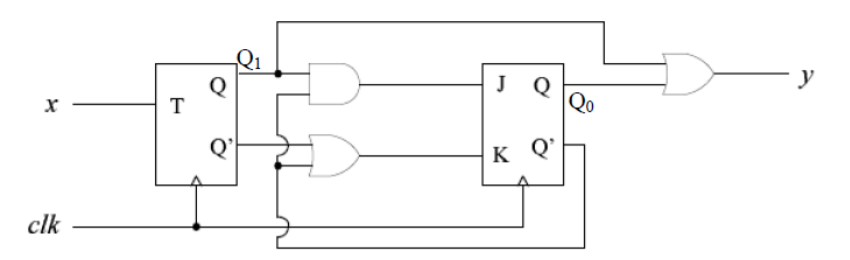
\includegraphics[scale=.8]{ExampleFFProblem.png}

\item Consider the following circuit.  What is the characteristic table for its output?

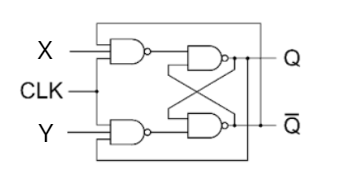
\includegraphics[scale=.8]{FlipFlopBehaviourProblemWithLabels.png}

\item What is the use of a half adder?  In what situation would this be used?

\item What is the characteristic table for the D flipflop?

\item Why is state S=1 R=1 undefined for an SR flipflop?

\item Is this 64-bit signed 2's complement number positive or negative? \\
1000011000101110111101001111100011101001111001100001101101010101

\item What is the purpose of a multiplexer?

\item What is the range of 8-bit signed 2's complement?

\item What is the difference between 1's complement and 2's complement?

\item What is a decoder used for in an ALU?

\item How do we implement memory in our circuits?

\item What is the disadvantage of a ripple-carry adder?

\end{enumerate}

\end{itemize}

\end{document}

